\chapter{Results and Evaluation}\label{results-and-evaluation}

\section{Evaluation}\label{evaluation}

Before the results of the presented proof-of-concept implementation are listed it needs to be clear what dimensions are important so that a distinction between good and bad results can be made.

A good reprojection map has several qualities that make it usable as an obstacle gridmap. First, it needs to be \textbf{timely}. That means that the time between the appearance of an object in the robot's path and it being mapped in an obstacle map needs to be small enough that the robot can still avoid collisions. The \textbf{false alarm rate}, representing false positive detections, needs to be low enough to not negatively influence the robot's navigation behaviour by making it circumnavigate phantom obstacles. Vice versa, the \textbf{missed target rate}, or false negative detection needs to be low, or the radar sensor will not bring an advantage over conventional obstacle sensors. The resulting map of course also needs to be \textbf{spatially correct}. This means that a detected obstacle is mapped at its true location. Otherwise, phantom obstacles or incorrectly sized obstacles will degrade map quality. The map becomes more useful if it contains \textbf{diverse types of obstacles}, and not just one class of objects, like walls. On the other hand, it should not contain \textbf{irrelevant information}, for example wall temperature is not interesting for obstacle detection. Lastly, only if the map is \textbf{comparable to other sensors} informed comparison can take place. For example, a glass wall is easily visible to the human eye, so their position in the radar reprojection map can be verified. But metal struts in walls, which, while not presenting an obstacle to the robot (vacuum robots usually are not designed to breach walls), could be useful landmarks for later slam applications, are not visible in other maps. Hence the quality of metal strut mapping can not be asserted, but only assumed based on human knowledge of where a wall's metal struts might be.

There are some classes of targets that are particularly interesting in the evaluation of results. The first one is stacks of \textbf{metal cans}, because they appear in many of the scans. This is a kind of artificial obstacle that was designed to have a high probability of visibility in both radar scans (the curved metal surface is very reflective from every direction) and lidar scans (the can towers are high enough to cross the laser beam, and wide enough to not be missed even in some distance). Another easy target are \textbf{walls}. They are easy to see in the lidar scan, and detections in the radar reprojection map can be easily compared. A special case of walls are \textbf{glass walls} or windows. They present an impenetrable obstacle in a robots path, but almost always, neither a laser scanner nor a vision sensor can detect them (see \cref{fig:rgbd_glasswall2}). Another real world obstacle that escapes lidar scans are \textbf{office chair legs}. While the pillar is visible with laser (green dot in \cref{fig:lidar_rgbd2}), the horizontally stretching legs and rollers are usually too low to be detected. In the same category of low profile obstacles are \textbf{cables} lying on the floor. A vacuum robot can easily entangle in them and get stuck. Lastly, it would be interesting to see negative obstacles including \textbf{cliffs} and dips. Today, robots need an extra set of sensors (usually IR distance sensors at the front of the robot, aiming at the floor) to detect this kind of obstacle very reliably.

\begin{figure}
  \begin{subfigure}[t]{.485\textwidth}
      \centering
      \def\svgwidth{\linewidth}
      \input{gfx/screenshots/rgbd_glasswall.pdf_tex}
      \caption{RGBD camera can not detect glass surface.}
      \label{fig:rgbd_glasswall2}
  \end{subfigure}%
  \hfill%
  \begin{subfigure}[t]{.485\textwidth}
      \centering
      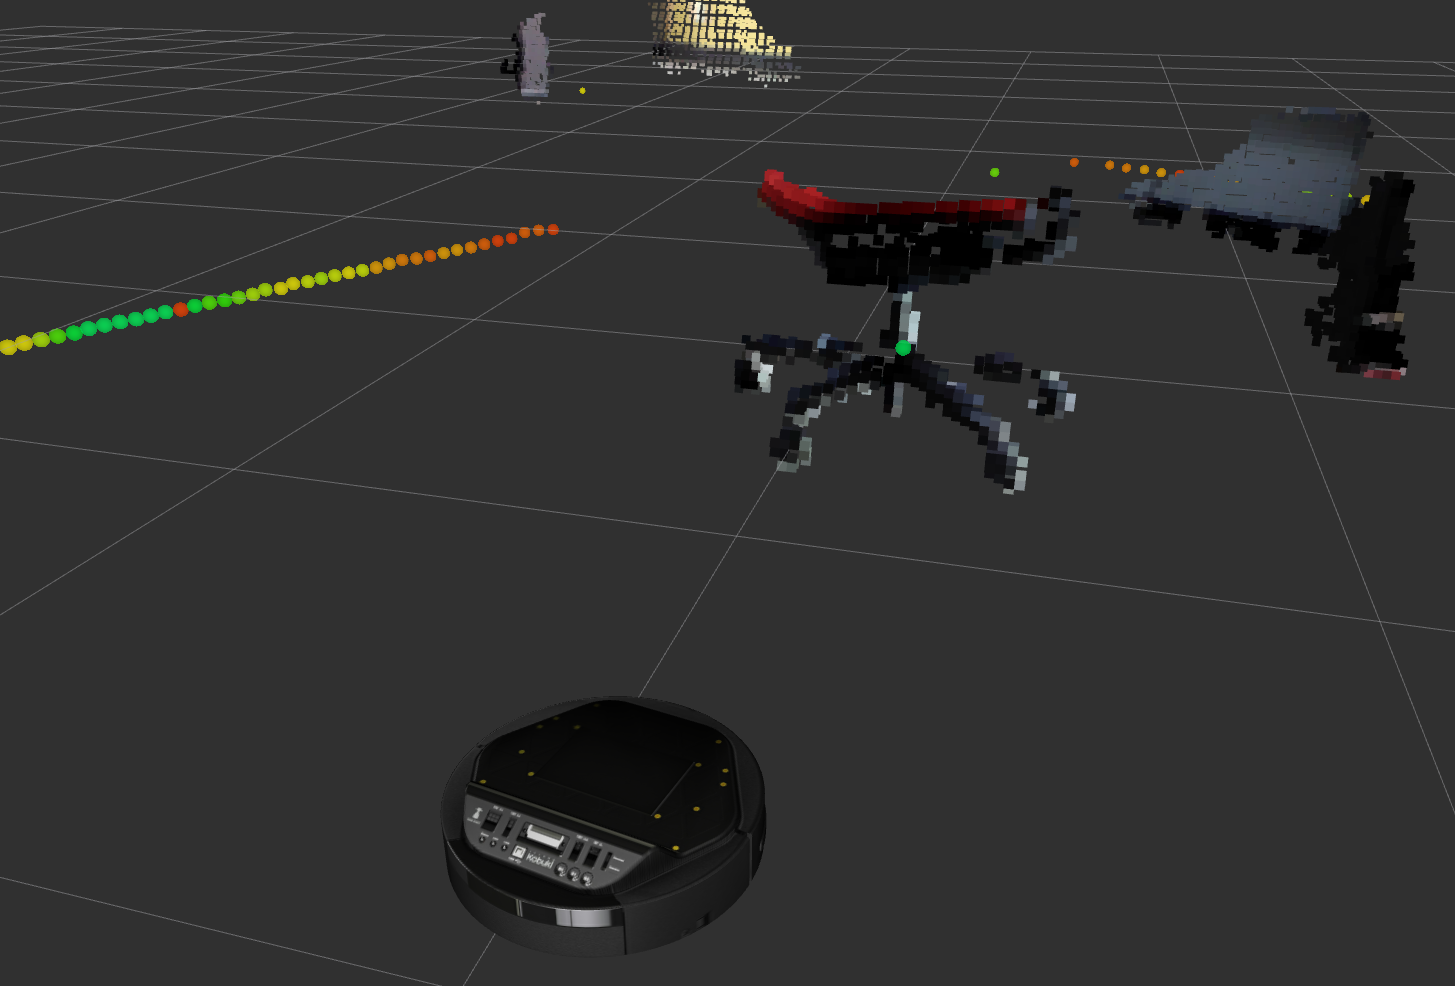
\includegraphics[max width=\textwidth]{gfx/screenshots/chair_laser_vs_rgbd}
      \caption{Laser fails to detect horizontal chair legs.}
      \label{fig:lidar_rgbd2}
  \end{subfigure}%
  \caption{Screenshots showing traditional sensor shortcomings.}
\end{figure}


\section{Results}\label{results}

During development of the reprojection method, over 30 scans were taken. The environment for the scans is the BSH office in the Bosch Research and Technology Center in Palo Alto, which is fairly representative of a typical office environment. It has carpet floors, desks, office chairs, walls, corridors, and even glass walls.

The 25 scans of this environment are assigned code names in alphabetical order for easy referencing. Only some exemplary results are shown here. The full list of scans and their parameters can be found in \cref{scans}.

\subsection{Plot Types}
The scans are presented through the following plot types.

\subparagraph{Input Energy}
This plot (e.g. top left of \cref{fig:pres3-i}) visualizes the preprocessed (i.e. oversampled, range and transmit crosstalk compensated) input energy of a scan. To understand the graph, it helps to first think of it as the stacked range profile of a range sensor that looks in a \ang{90} angle to the right of the robot. The x-axis represents down-range (in \si{m}), which is the range axis in the 1D range profile as extracted from the FMCW beat frequency (see \cref{fig:rawbeat_f} for an example). Each range profile line's echo intensity (shown on the y-axis in \cref{fig:rawbeat_f}) is visualized in a logarithmic \texttt{hcparula}\footnote{\texttt{hcparula} is a monotonic, linear-grayscale intensity colormap with enhanced contrast. It is available at \url{https://www.mathworks.com/matlabcentral/fileexchange/61768}} color scale. The unit is \si{dB Vrms}. These range lines are stacked over the Y-axis direction, which is the cross-range dimension. This dimension shows how far the radar sensor has traveled from the scan's origin (i.e. mileage, in \si{m}). If the radar was moved at a constant velocity, it can be thought of as the time axis, however denoting and processing it as mileage has the benefit of radar velocity independence. Note that this plot does not show any information on where (at which angle) a target is, but only at what distance it is. Target peaks appear and disappear over the course of the y-axis, because they enter or leave the radar antenna's field of view.

\subparagraph{Doppler estimation}
To calculate reprojection angles, a target's Doppler speed must be estimated. This graph (e.g. \cref{fig:pres3-d}) shows the estimation from the peak gradient algorithm: Every detected peak has a certain speed associated with it. This speed is plotted as color over the FWHM around the peak's location in down-range/cross-range space. The color follows a symmetric linear pink/white/green color scale\footnote{Specifically, \texttt{PiYG} via the \texttt{cbrewer} function, which is available at \url{https://www.mathworks.com/matlabcentral/fileexchange/34087}}. The estimated Doppler speed is not shown in its smoothed version, which is averaged over cross range as described in \cref{raw-data-smoothing} and peak FWHM as described in \cref{peaks-overlaps-at-crossing-target-arcs}. The background of the graph is dark grey to make sure the white middle of the color scale is visible, as well as to help highlight where Doppler peaks were actually detected.

\subparagraph{DOA estimation}
The third input graph (e.g. \cref{fig:pres3-doa}) shows DOA data as estimated in \cref{doa-implementation}, which in the current implementation is solely used to resolve the left-right reprojection angle ambiguity in the forward-looking geometry (see \cref{geometry-for-the-general-case}). The (darkened) graph background visualizes the phase difference of the oversampled complex analytic input signal of both receiving radar antennas. Similar to the Doppler graph, DOA information over detected peaks is smoothed over cross-range and each peak's FWHM. The color is the same symmetric pink/white/green as the Doppler plot. The color scale is from $-\pi/3$ to $\pi/3$ radian; values above or below are clipped (but this happens only for the noisy background signal).

\subparagraph{Reprojection map}
This is the main output of the reprojection mapping implementation, as described in \cref{reprojection-mapping}. The graph (e.g. \cref{fig:pres3-r}) shows a top-view 2D map, with the origin (0,0) at the scan starting point. Axes are in \si{m}. The color scale is again \texttt{hcparula}, with echo intensities in \si{dBVrms}. The red line shows the radar motion path.

\subparagraph{Reprojection map overlay}
If the \texttt{/map} is available for a scan, this graph (e.g. \cref{fig:pres3-l}) shows the reprojection map overlaid over the lidar occupancy gridmap as described in \cref{output}. The lidar map has a grayscale colormap, where black means occupied, white means clear, and anything in between shows occupancy probability. Uncharted, unknown values are a ``tasteful blueish greenish grayish color''\footnote{Legal \texttt{-1} value from \url{http://docs.ros.org/jade/api/rviz/html/c++/map\_\_display\_8cpp\_source.html\#l00212}}. The red path is again the radar motion path.

\subsection{Exemplary Results}
Exemplary results are shown in \cref{fig:pres1,fig:pres2,fig:pres3,fig:pres4}. More result plots can be found in \cref{scans}.

\begin{figure}[htbp]
    \centering
    \begin{subfigure}{.95\textwidth}
        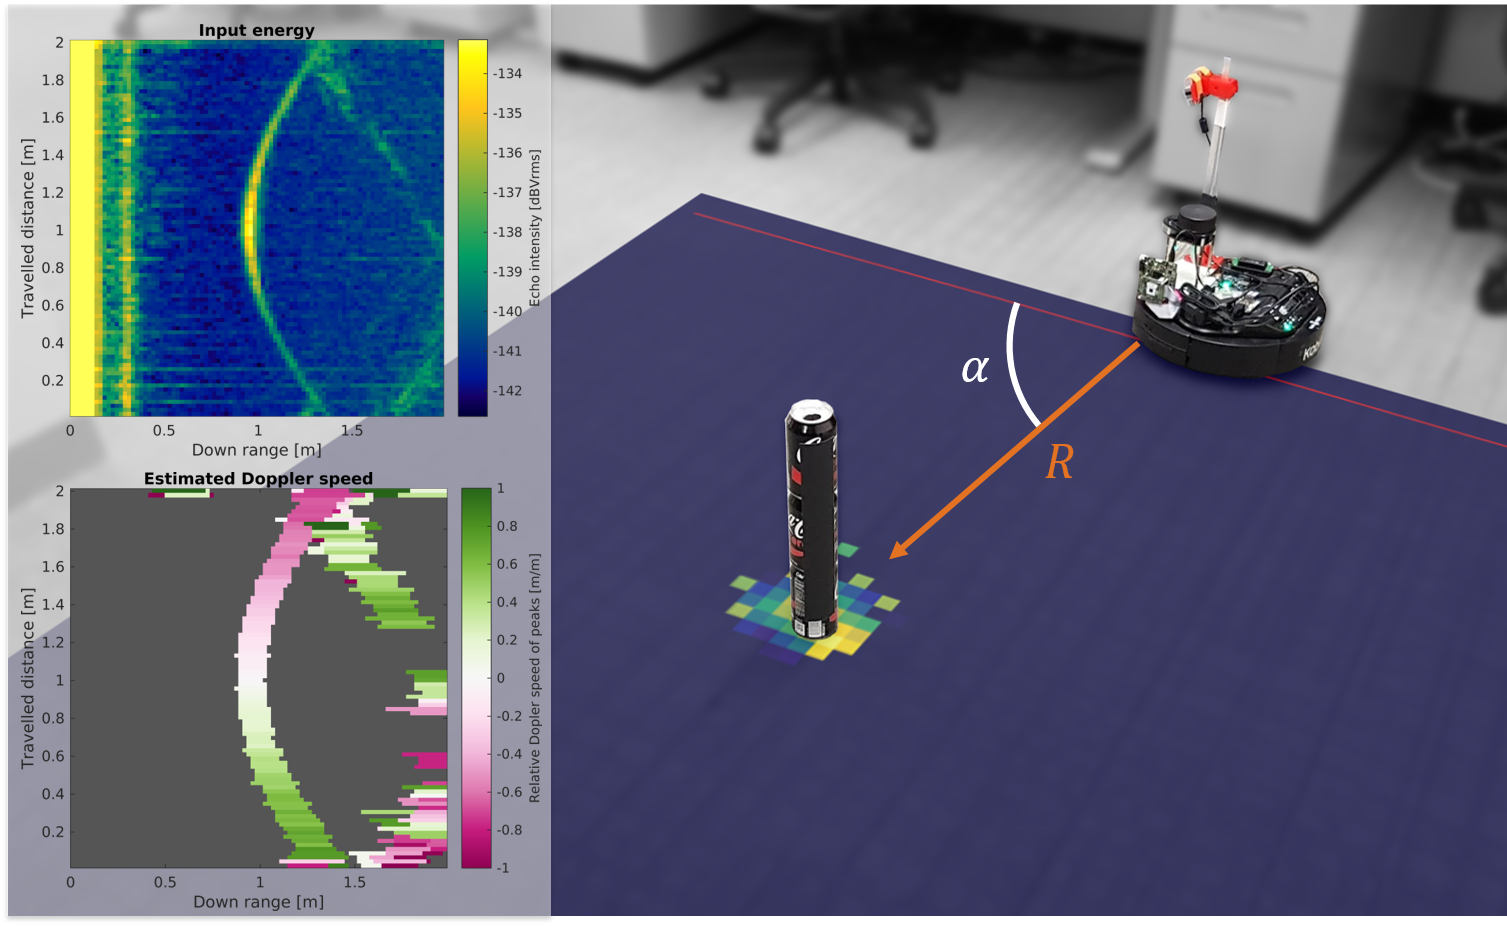
\includegraphics[max width=\textwidth]{gfx/diagrams/presentationscan1.png}
        \caption{A simple example scan with only one major (point) target. The range cell migration arc is clearly visible in both input energy (top left) and Doppler estimation (bottom left). The reprojection map is overlaid on the floor of the scene picture on the right.}
        \label{fig:pres1}
    \end{subfigure}\medskip\\
    \begin{subfigure}{.95\textwidth}
        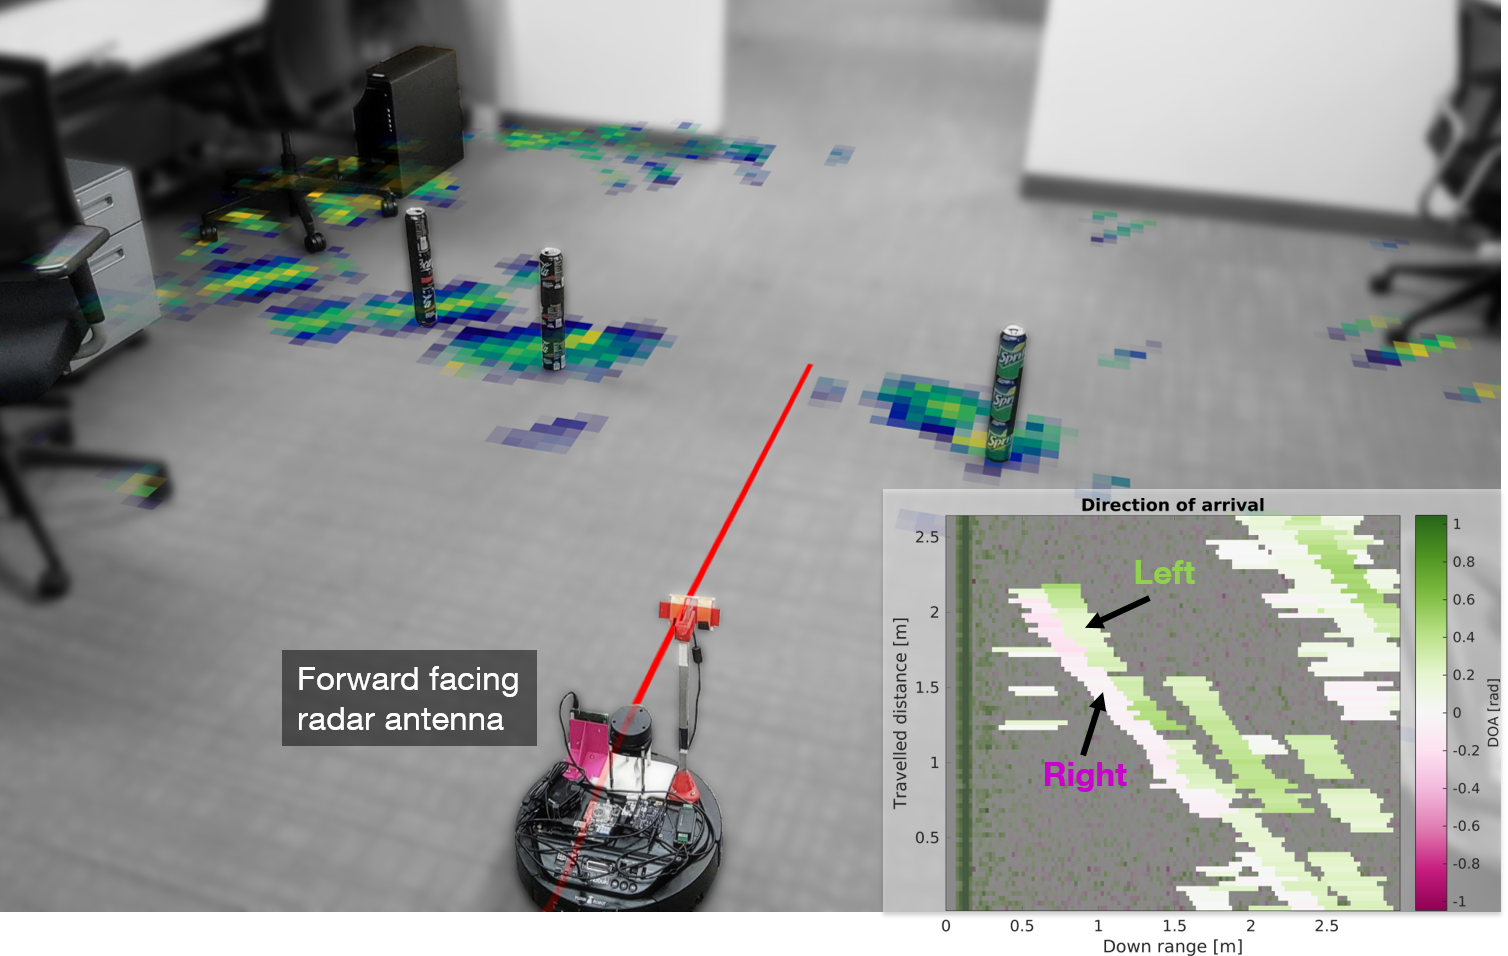
\includegraphics[max width=\textwidth]{gfx/diagrams/presentationscan_2.png}
        \caption{This example scan shows how the angle sign ambiguities discussed in \cref{geometry-for-the-general-case} are resolved with DOA values (bottom right). The reprojection map is overlaid on the floor of the scene picture on the right and shows that targets left and right of the motion path (red line) were clearly separated.}
        \label{fig:pres2}
    \end{subfigure}
    \caption{Examples of simple side- and forward facing radar antenna.}
\end{figure}


\begin{figure}[htbp]
    \centering
    \begin{subfigure}[t]{.3\textwidth}
        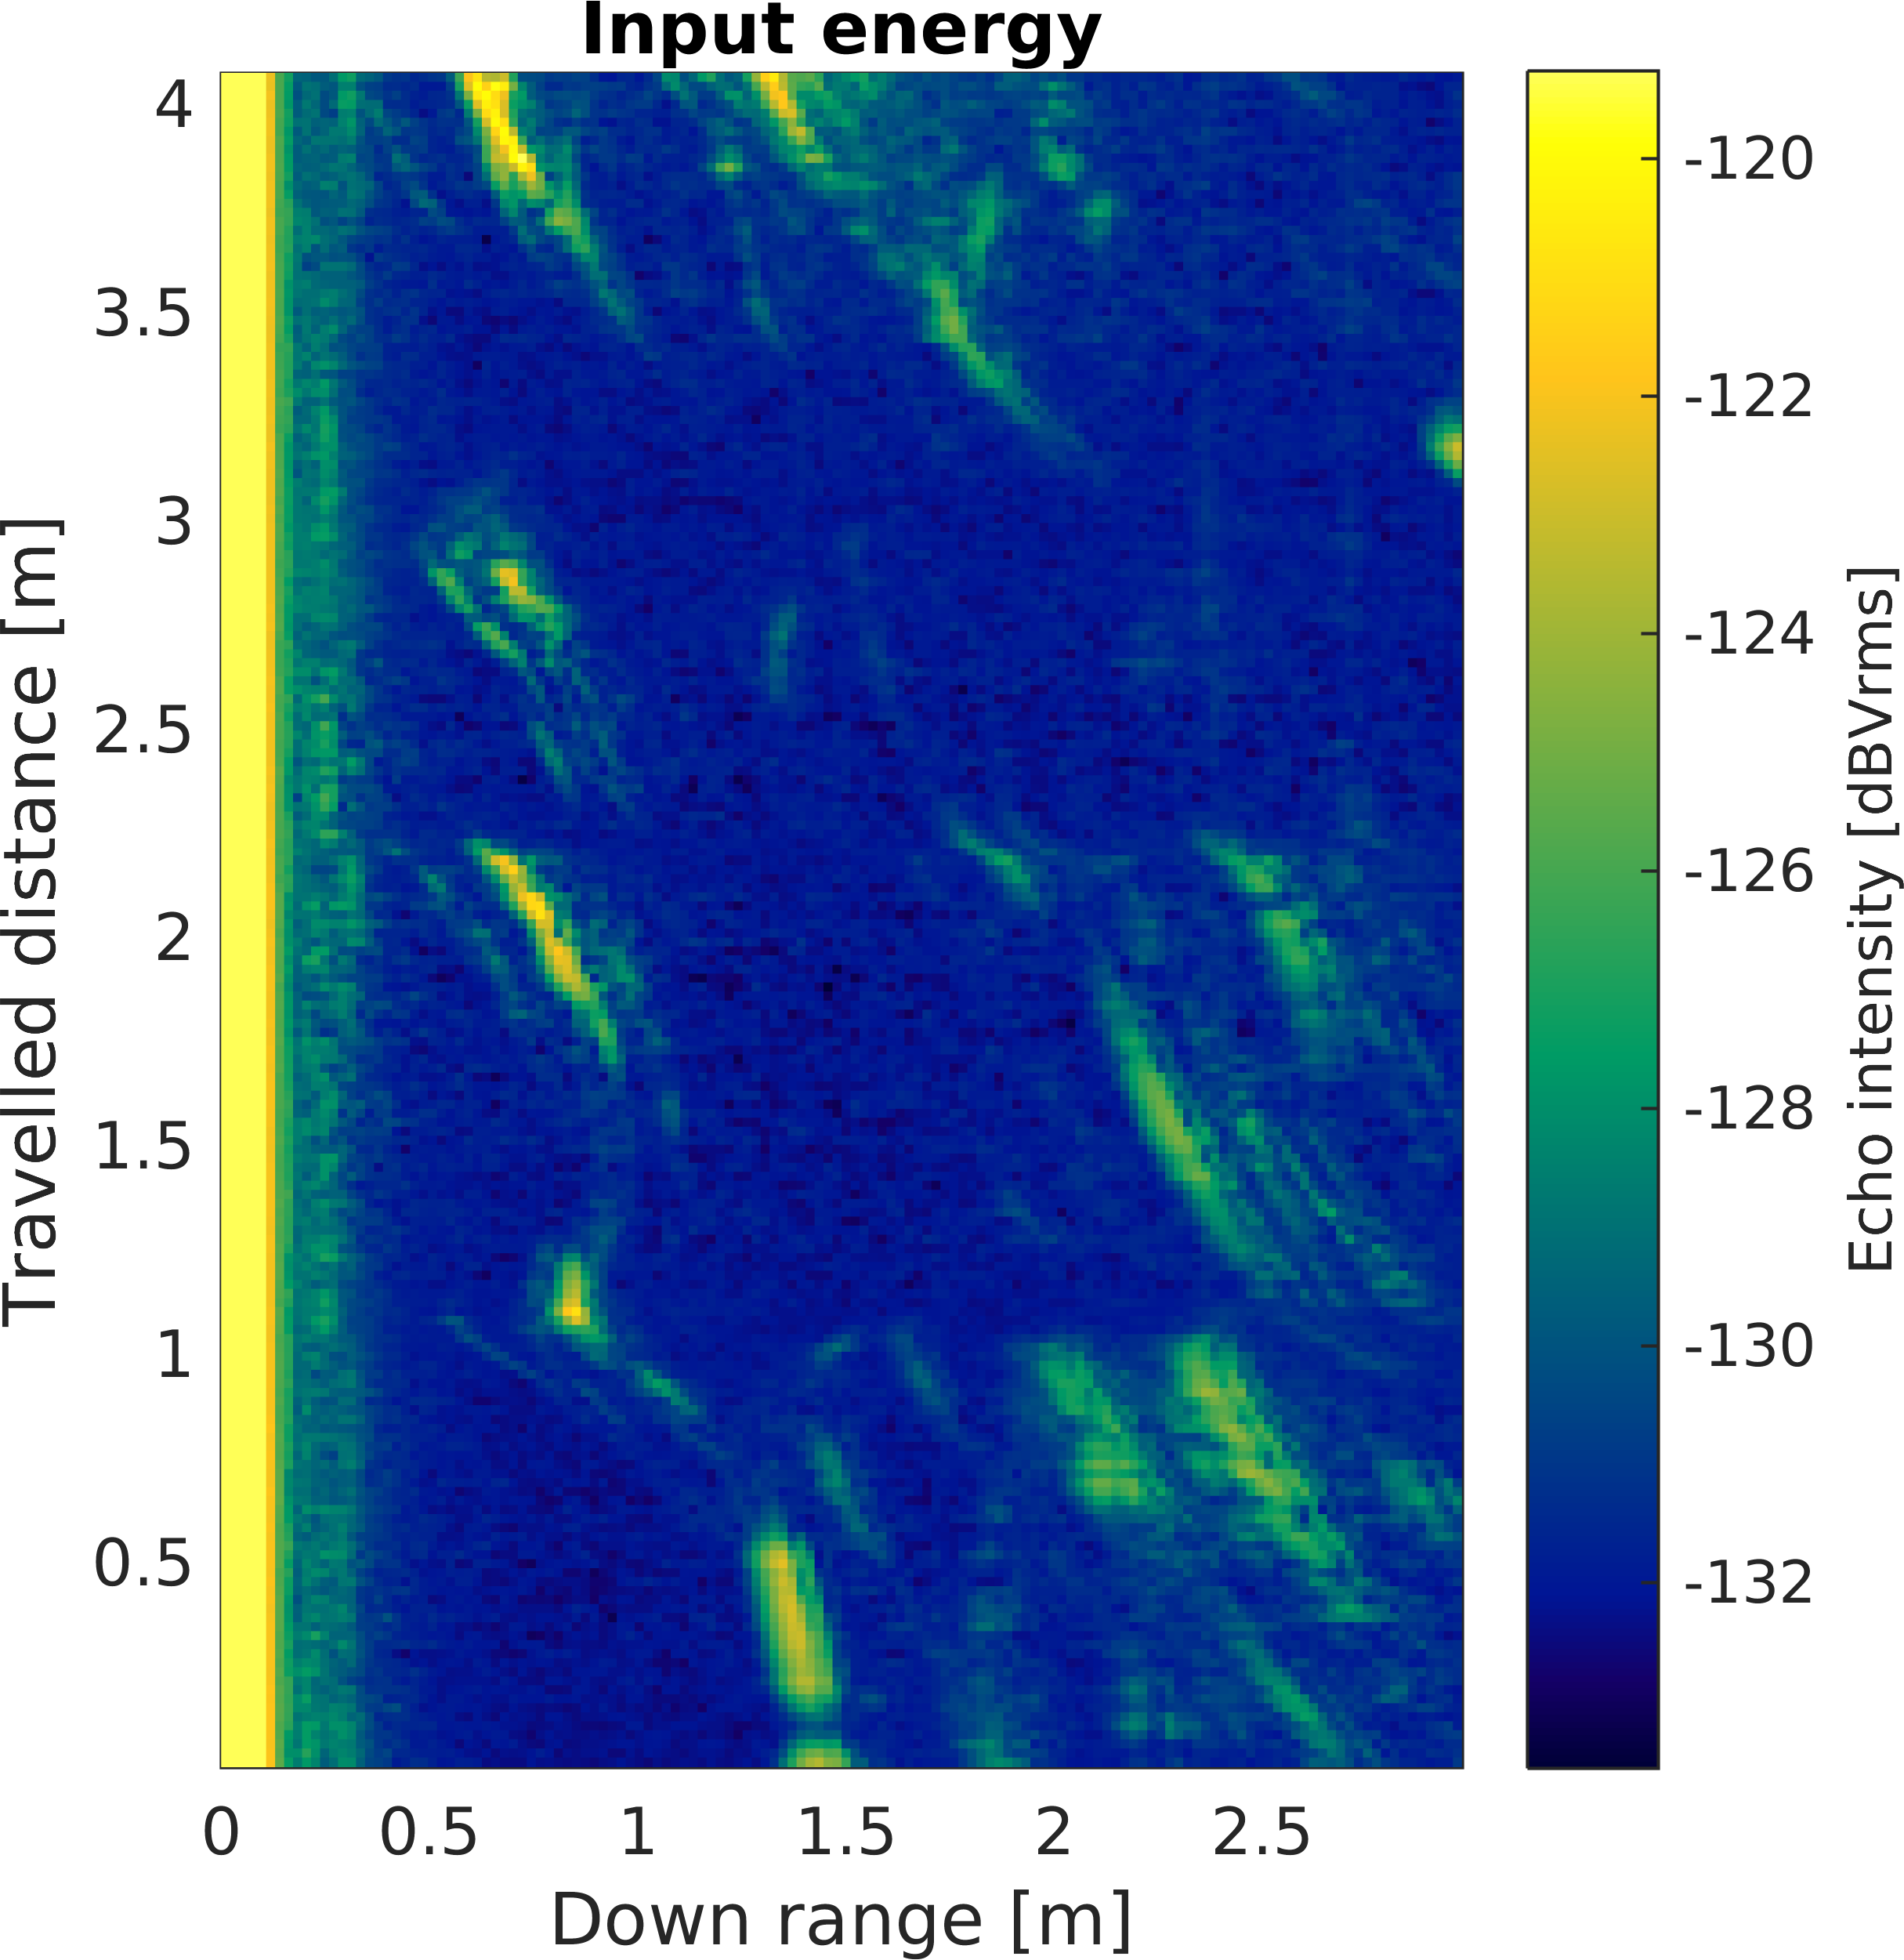
\includegraphics[max width=\linewidth]{gfx/figures/t_input.png}
        \caption{Input energy.}
        \label{fig:pres3-i}
    \end{subfigure}%
    \hfill%
    \begin{subfigure}[t]{.3\textwidth}
        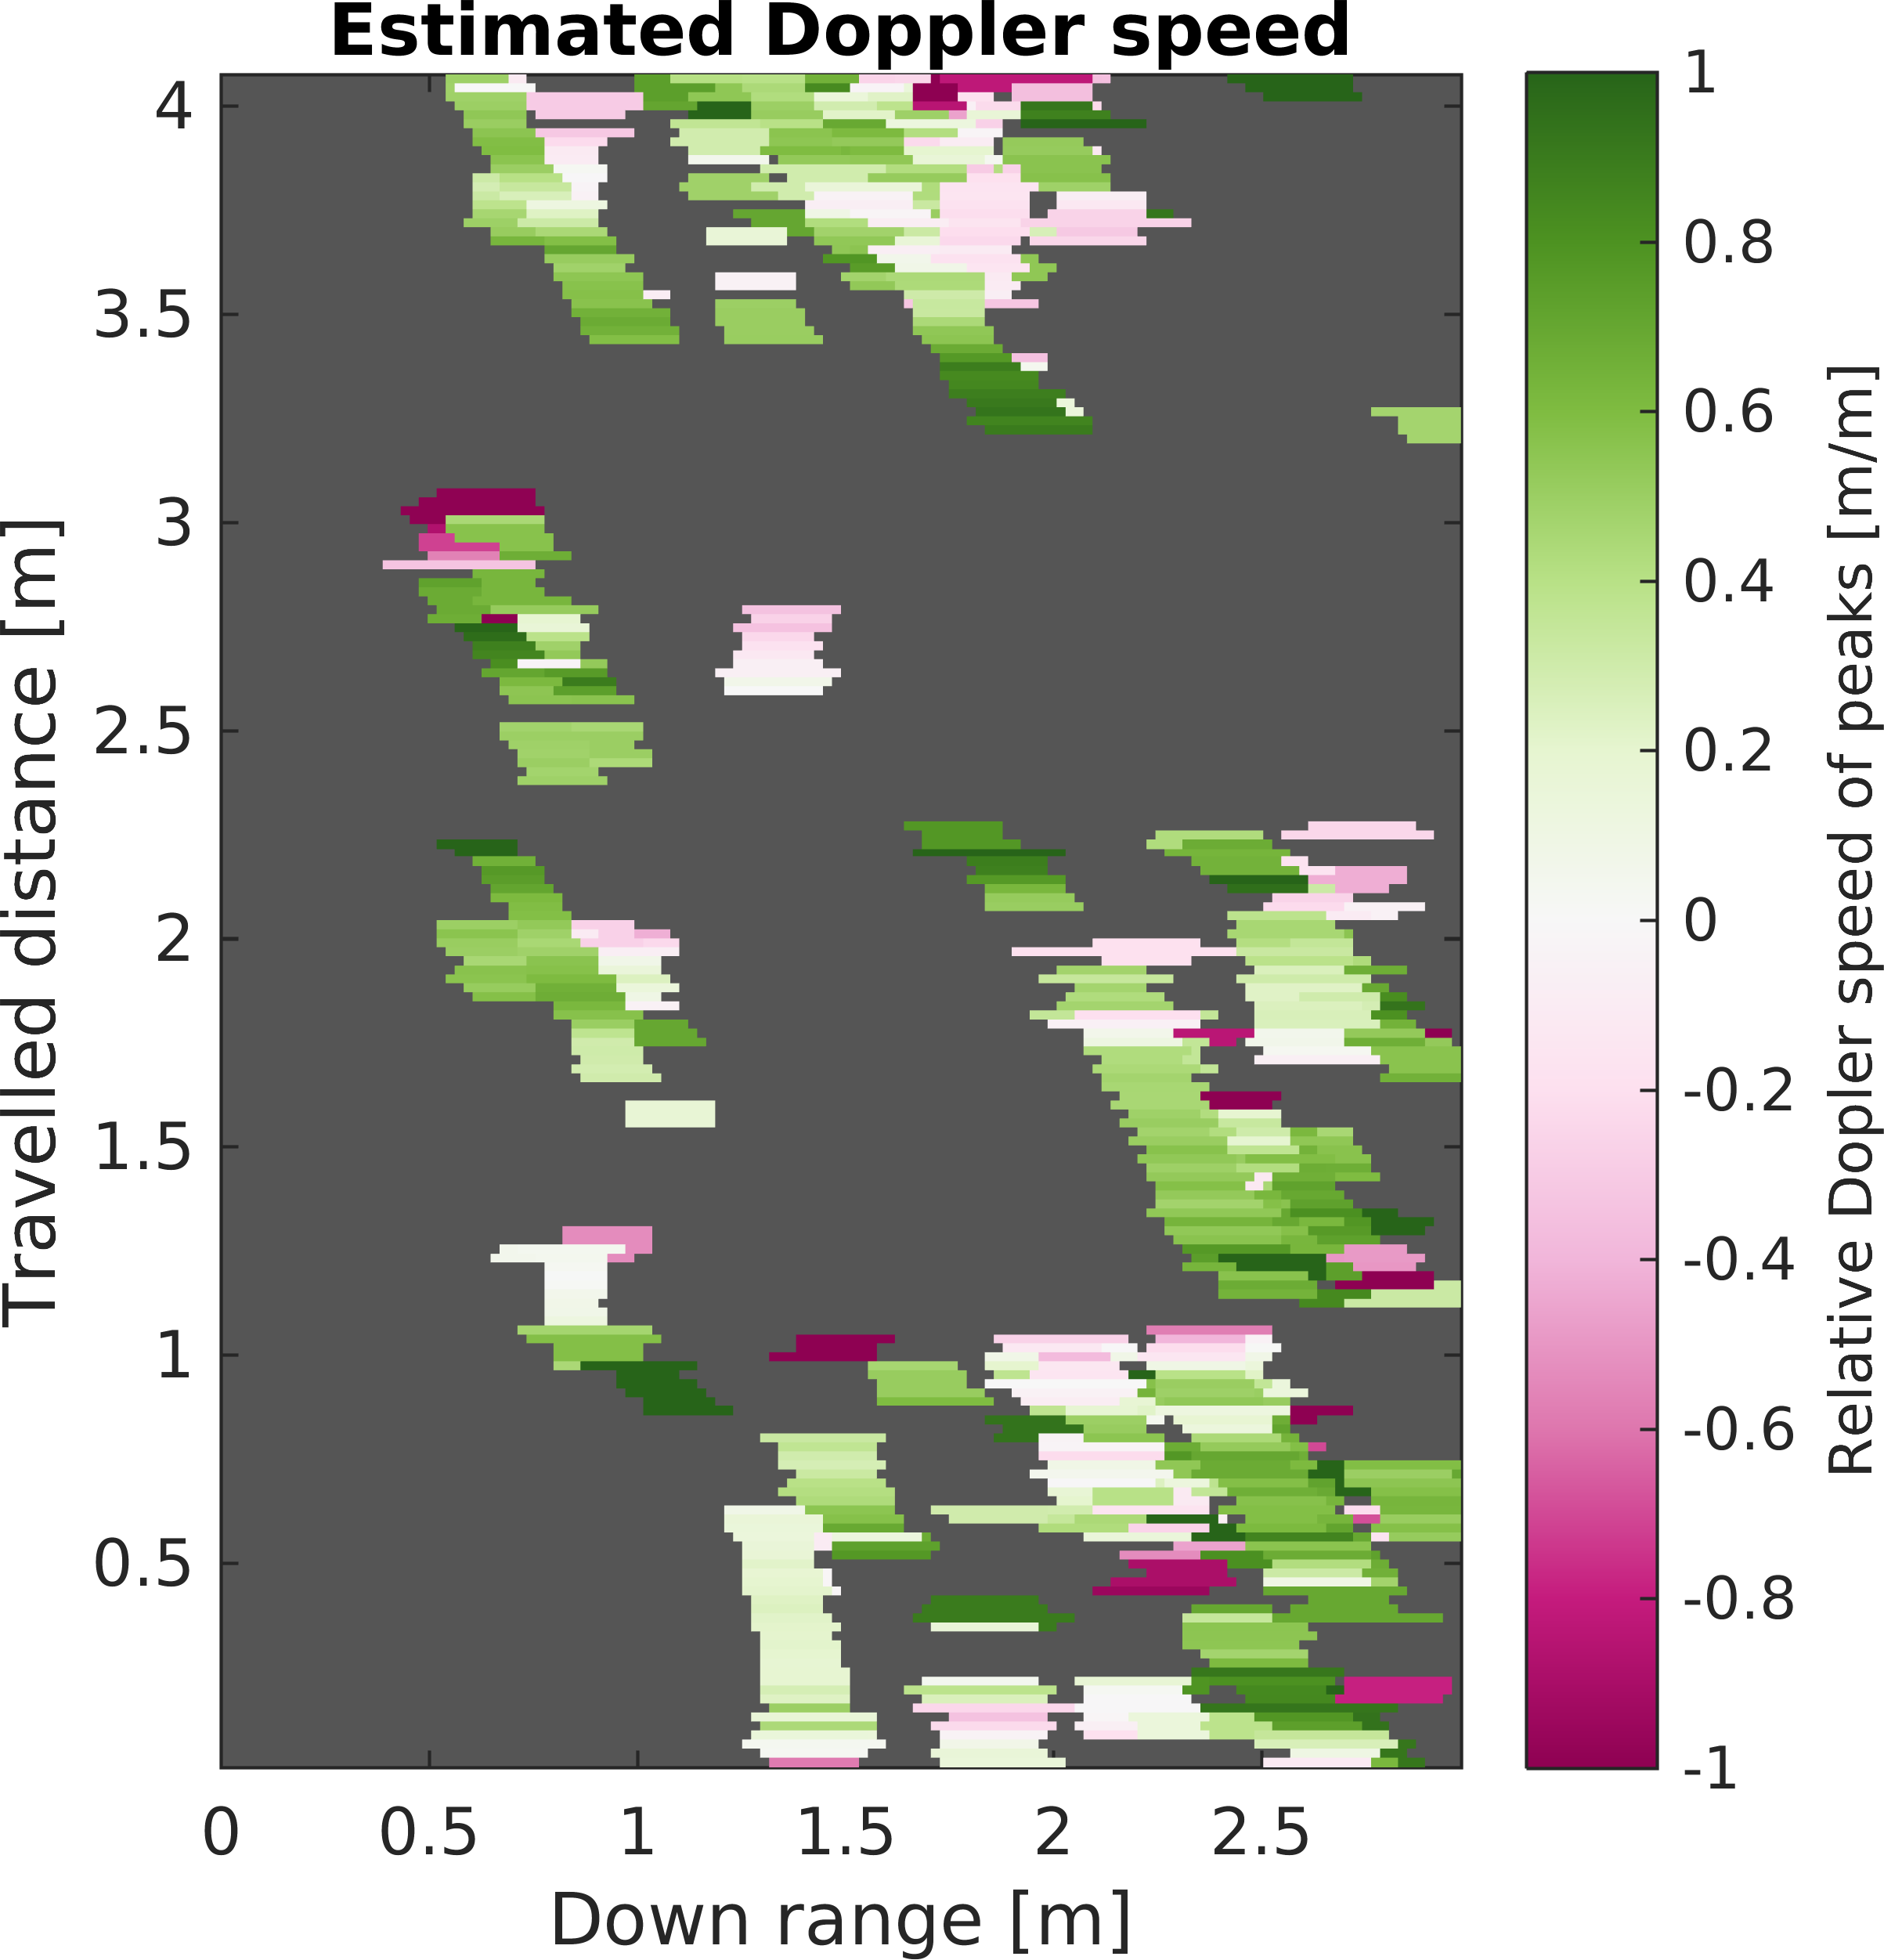
\includegraphics[max width=\linewidth]{gfx/figures/t_doppler.png}
        \caption{Doppler estimation.}
        \label{fig:pres3-d}
    \end{subfigure}%
    \hfill%
    \begin{subfigure}[t]{.3\textwidth}
        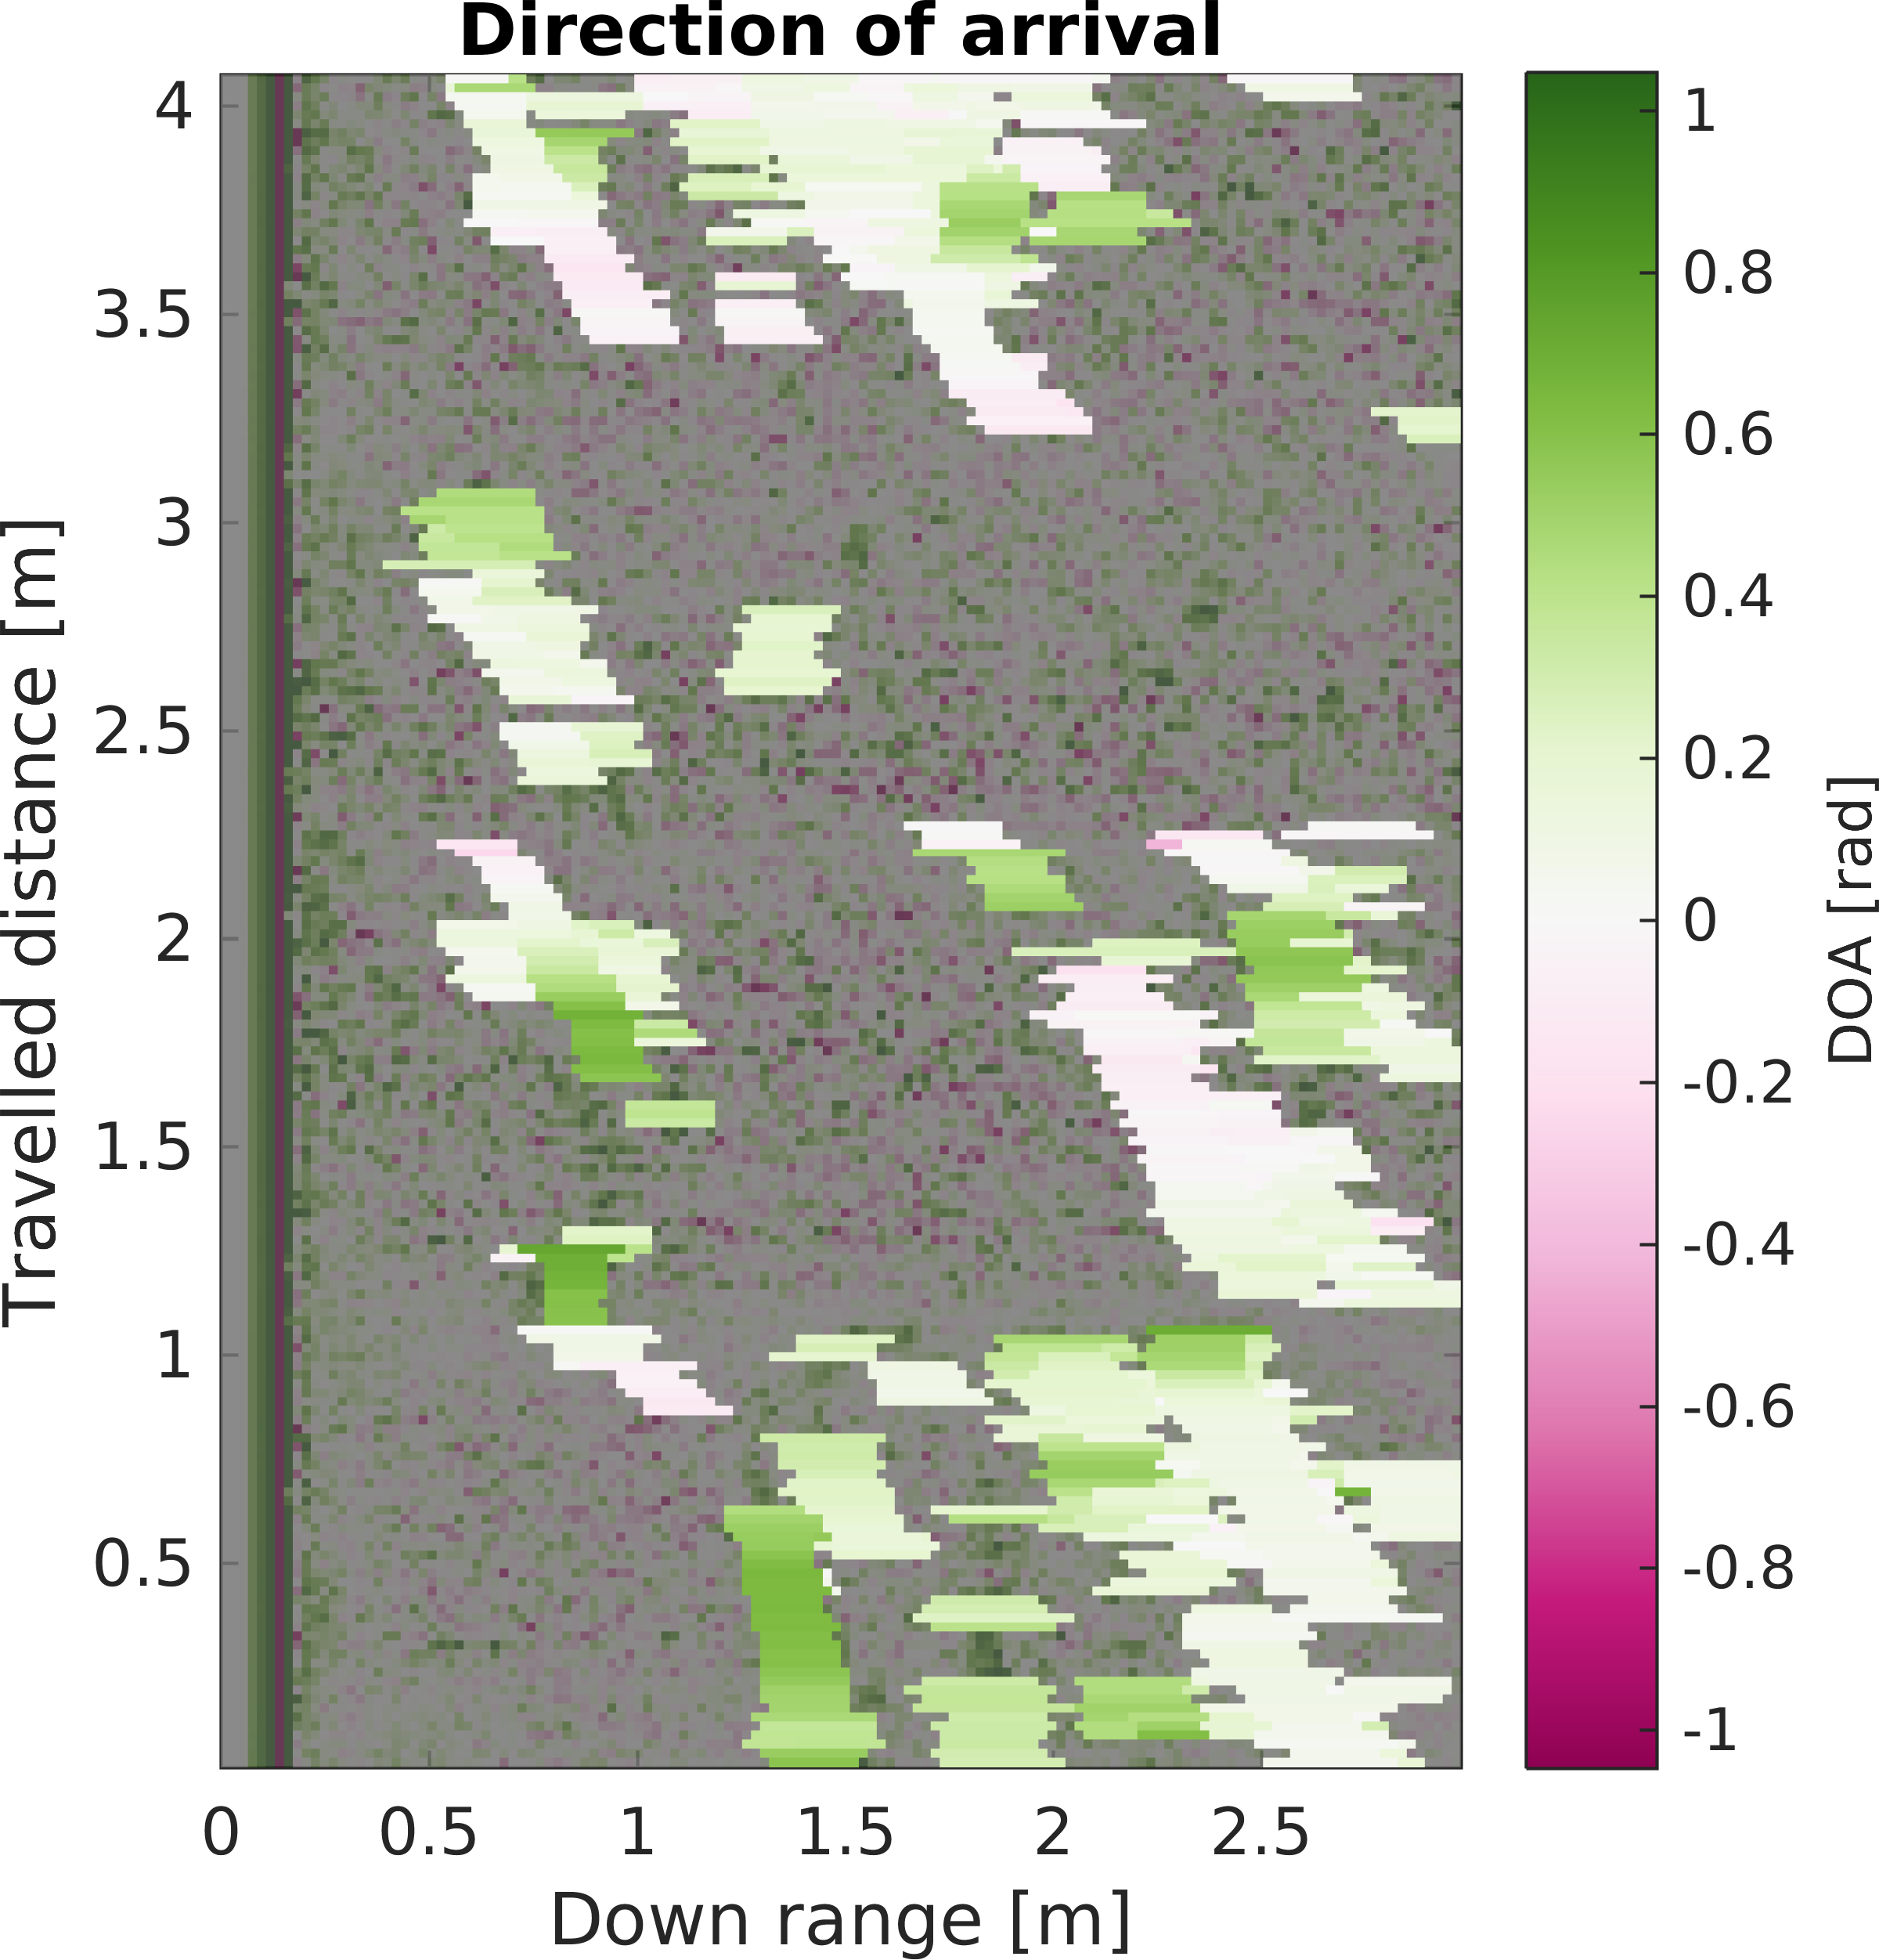
\includegraphics[max width=\linewidth]{gfx/figures/t_doa.png}
        \caption{DOA estimation.}
        \label{fig:pres3-doa}
    \end{subfigure}\medskip\\
    \begin{subfigure}[t]{.45\textwidth}
        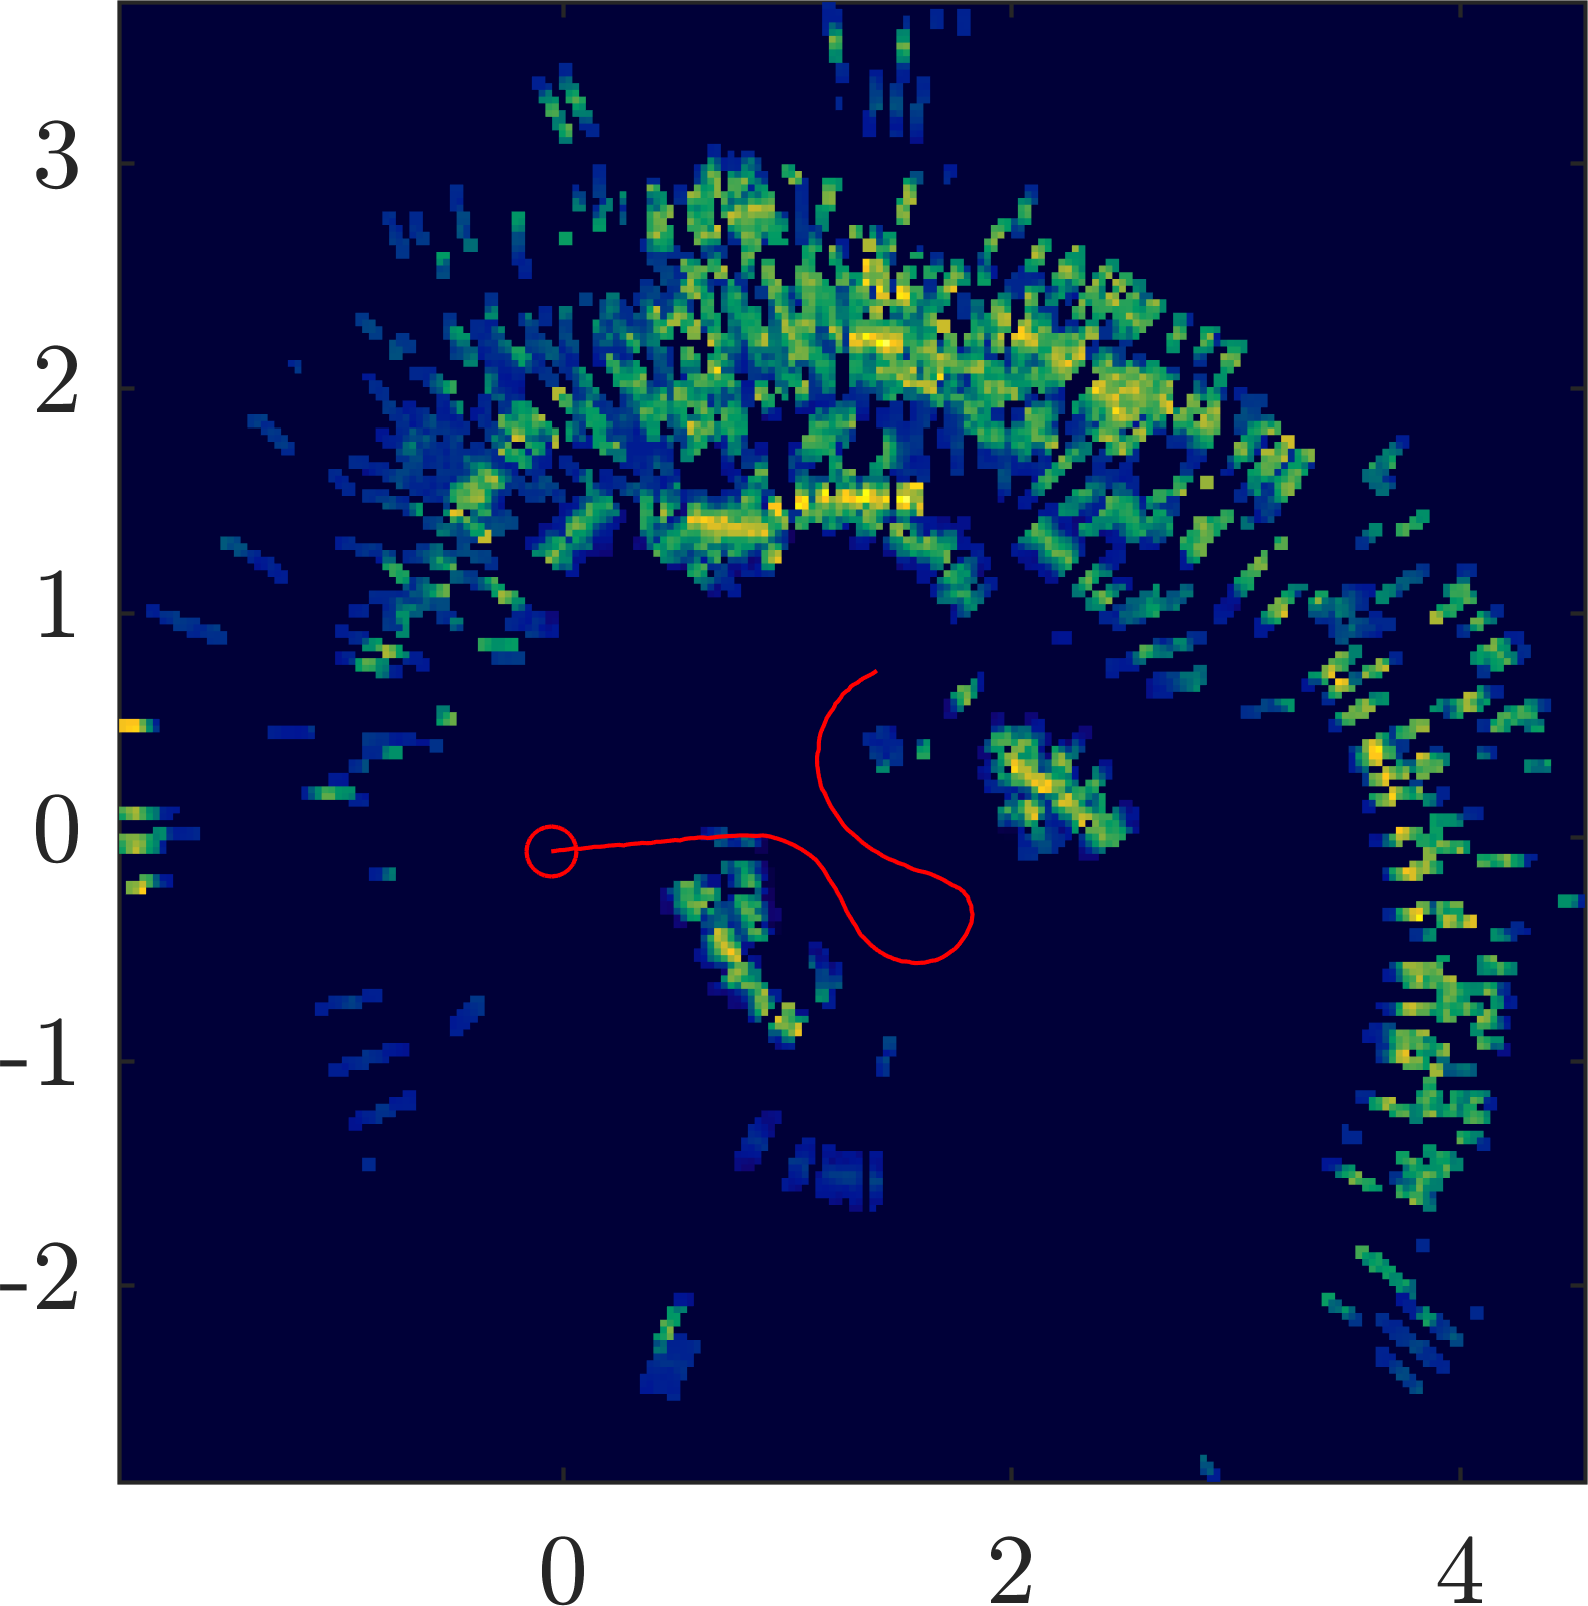
\includegraphics[max width=\linewidth]{gfx/results/torturechamber_reprojection.png}
        \caption{Reprojection map.}
        \label{fig:pres3-r}
    \end{subfigure}%
    \hfill%
    \begin{subfigure}[t]{.45\textwidth}
        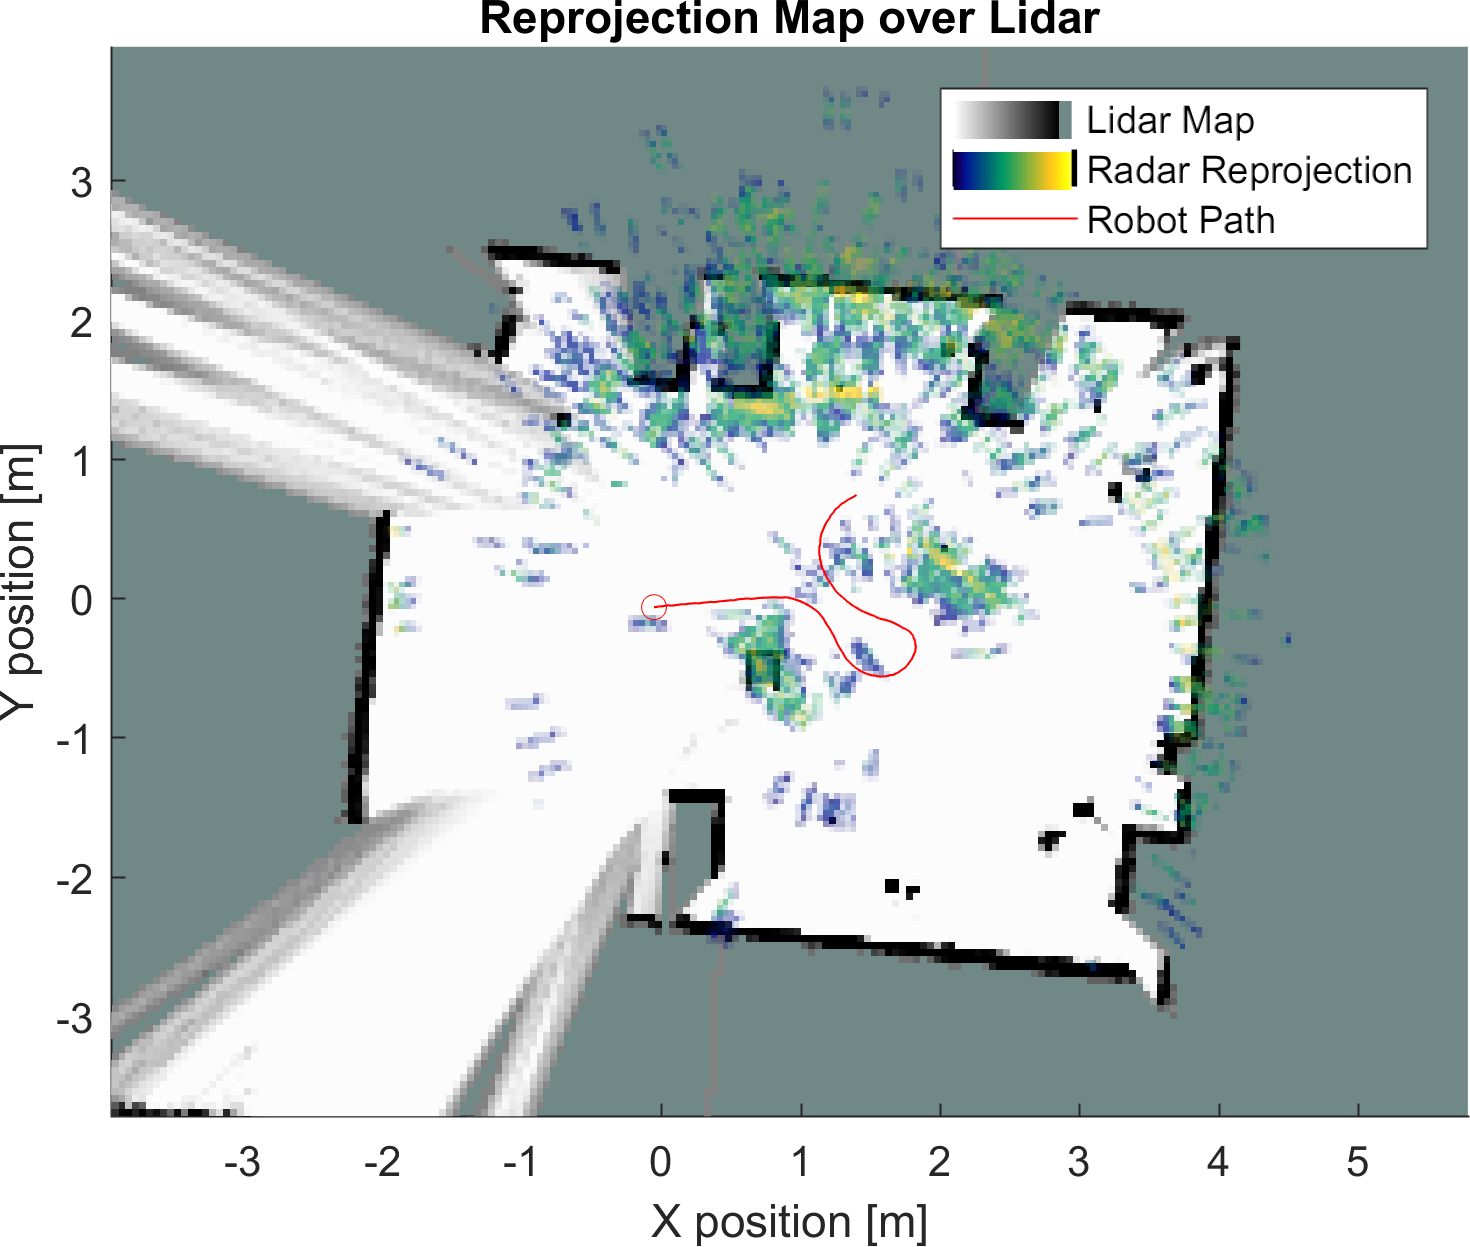
\includegraphics[max width=\linewidth]{gfx/results/torturechamber_map.png}
        \caption{Reprojection map overlaid over lidar-based slam occupancy gridmap.}
        \label{fig:pres3-l}
    \end{subfigure}\medskip\\
    \begin{subfigure}{\textwidth}
        \includegraphics[max width=\linewidth]{gfx/diagrams/presentationscan_torture.png}
        \caption{Reprojection map overlaid on a picture of the scene.}
        \label{fig:pres3-3d}
    \end{subfigure}
    \caption{Several plots representing the Torture Chamber scan.}
    \label{fig:pres3}
\end{figure}

\begin{figure}[htbp]
    \centering
    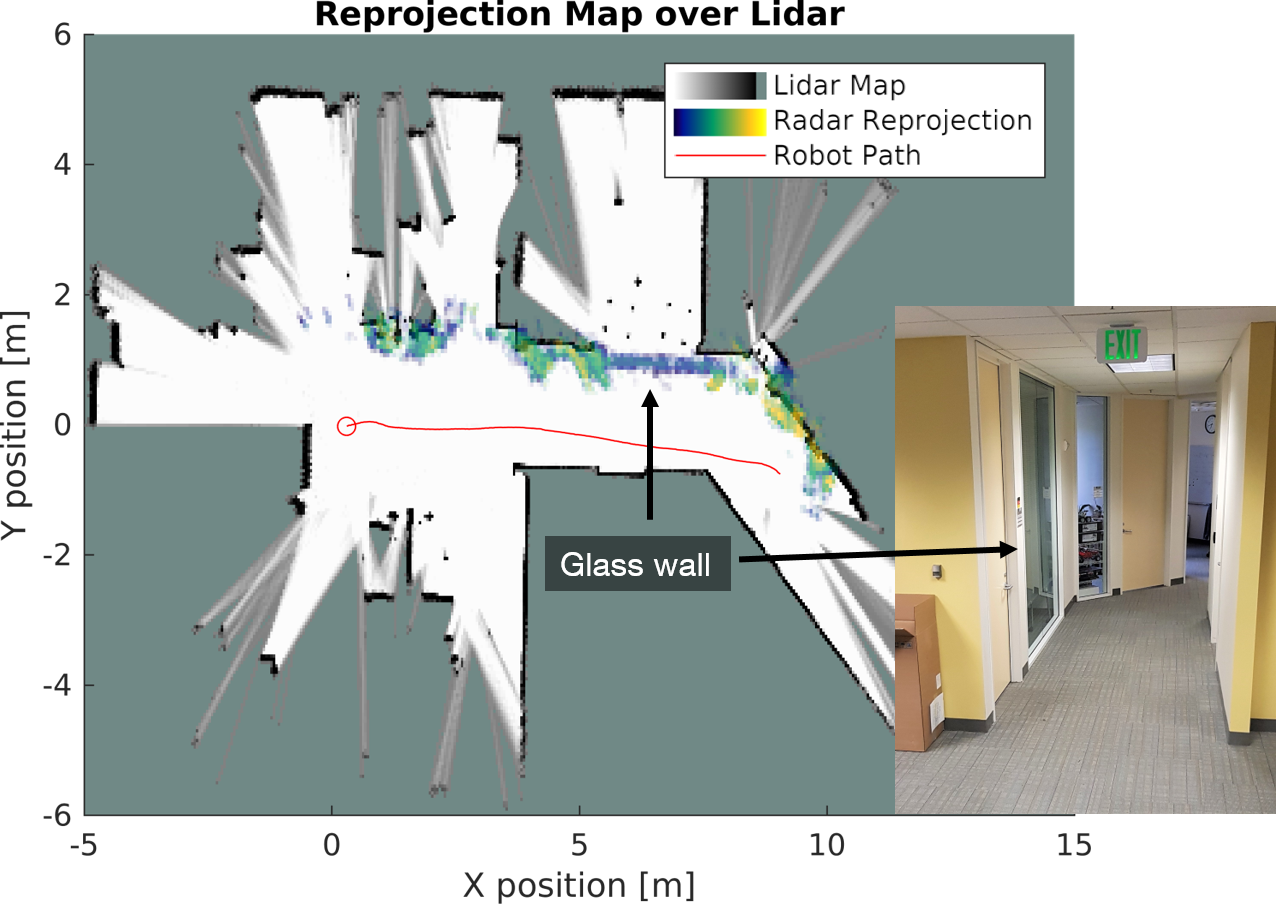
\includegraphics[max width=\textwidth]{gfx/diagrams/pres4.png}
    \caption{This example scan shows the reprojection map overlay of the Underground scan. The grayscale laser slam mapped the room behind the depicted corridor's glass wall, but it does not the glass wall itself. The radar reprojection map however prominently features the obstacle.}
    \label{fig:pres4}
\end{figure}